% Week 1 — Revision of mathematics, told as business decisions
% Build: latexmk -pdf week01.tex   (or pdflatex twice)
% Half lab, half slides: LAB frames are the cue to switch to session.ipynb; PAPER frames to drills.md.
\documentclass[aspectratio=169,11pt]{beamer}
\usetheme[progressbar=frametitle,numbering=fraction,block=fill]{metropolis}
\usepackage[T1]{fontenc}
\usepackage[utf8]{inputenc}
\usepackage{booktabs}
\usepackage{pgfplots}
\pgfplotsset{compat=1.18,scaled ticks=false}
\usetikzlibrary{arrows.meta,positioning}
\usepackage{hyperref}

\definecolor{navy}{HTML}{2471A3}
\definecolor{brick}{HTML}{C0392B}
\definecolor{leaf}{HTML}{1E8449}
\definecolor{slate}{HTML}{7F8C8D}
\setbeamercolor{alerted text}{fg=brick}
\setbeamercolor{example text}{fg=leaf}

% ---------- helpers ----------
\newcommand{\bet}[1]{\begin{alertblock}{Bet before we compute}#1\end{alertblock}}
\newcommand{\board}[1]{\begin{exampleblock}{Board sentence}#1\end{exampleblock}}
\newcommand{\labframe}[3]{% #1 notebook section, #2 title, #3 body
  {\setbeamercolor{background canvas}{bg=navy}\setbeamercolor{normal text}{fg=white}\usebeamercolor[fg]{normal text}
  \begin{frame}[plain]
    \vspace{0.6em}{\large\textbf{LAB}\quad\texttt{session.ipynb} #1}\par\vspace{0.4em}
    {\Large #2}\par\vspace{1em}#3
  \end{frame}}}
\newcommand{\paperframe}[2]{% #1 drills, #2 minutes
  {\setbeamercolor{background canvas}{bg=slate!15}
  \begin{frame}[plain]
    \vspace{0.6em}{\large\textbf{PAPER}\quad\texttt{drills.md}}\par\vspace{0.4em}
    {\Large #1}\par\vspace{0.6em}{#2 minutes. Show all work, exam style. I come round.}
  \end{frame}}}
\newcommand{\clipframe}[3]{% #1 image basename, #2 overlay count spec, #3 mp4 name
  {\setbeamercolor{background canvas}{bg=black}\setbeamercolor{normal text}{fg=white}\usebeamercolor[fg]{normal text}
  \begin{frame}[plain]
    \centering #2
    \vspace{-0.2em}\par{\footnotesize \href{run:../../anim/out/#3}{$\blacktriangleright$ play \texttt{\detokenize{#3}}}}
  \end{frame}}}

\title{Revision of mathematics,\\told as business decisions}
\subtitle{MBA03 Research \& Quantitative Business Methods --- Week 1}
\author{Niccolò Salvini}
\institute{European School of Economics, Florence}
\date{Thursday 24 September 2026}

\begin{document}
\maketitle

% ------------------------------------------------------------------
\begin{frame}{Where the first five weeks go}
  \begin{columns}[T]
  \begin{column}{0.58\textwidth}
    \begin{tabular}{@{}lll@{}}\toprule
    Wk & Date & What you will be able to do by hand \\ \midrule
    1 & 24 Sep & equations, systems, quadratics, logs \\
    2 & 1 Oct & read a function; limits; the derivative \\
    3 & 8 Oct & study a function; optimise; integrate \\
    4 & 15 Oct & interest, discounting, NPV \\
    5 & 22 Oct & bonds, duration, convexity; mock exam \\ \bottomrule
    \end{tabular}
  \end{column}
  \begin{column}{0.40\textwidth}
    \textbf{Two things count.}\\[0.3em]
    Midterm (25\%): a report to a Board built on the study of a cost, a revenue and a profit function. Due 1 Nov.\\[0.5em]
    Final exam (75\%): 3 hours, paper, calculator. One of five questions is pure calculus: integrals, limits, recovering a function from its derivative.
  \end{column}
  \end{columns}
  \vspace{0.6em}
  \alert{Every technique in this room is here because one of those two asks for it. I will tell you which one, every time.}
\end{frame}

\begin{frame}{The shape of an exam item}
  \begin{columns}[T]
  \begin{column}{0.5\textwidth}
    \textbf{Same form as the final, different numbers:}
    \begin{align*}
      &\int \frac{x^{5} - 3x^{3} + 2}{x^{2}}\,dx \\[0.3em]
      &\lim_{x \to 1^{+}} \frac{(x-1)^{2}}{x - x^{2}} \\[0.3em]
      &f'(x) = 6x^{2} - 2x,\;\; f(1) = 4 \;\;\Rightarrow\;\; f(x) = ?
    \end{align*}
  \end{column}
  \begin{column}{0.5\textwidth}
    Today we do none of this. Today we make sure that when we get there, the \emph{algebra} underneath --- dividing term by term, factoring, solving for an unknown, handling a log --- is not what slows you down.\\[0.8em]
    Everything today is a question the founder of a small firm actually has to answer.
  \end{column}
  \end{columns}
\end{frame}

\begin{frame}{The case: Arno Bikes}
  \centering
  \begin{tabular}{@{}ll@{}}\toprule
    e-bike assembler, Florence & \\ \midrule
    Fixed cost & \texteuro 60{,}000 per month (rent, salaries, insurance) \\
    Variable cost & \texteuro 400 per bike (parts, packaging) \\
    List price & \texteuro 1{,}000 per bike \\ \bottomrule
  \end{tabular}
  \vspace{1em}

  Four questions from the founder, one per block:\\[0.3em]
  \textbf{A.} How many bikes before I stop losing money? \quad
  \textbf{B.} How many bikes should I make? \\
  \textbf{C.} How long until revenue doubles? \quad
  \textbf{D.} Is this battery cell within spec?
\end{frame}

% ================================================================== A
\section{A. Launch or not? --- linear equations and systems}

\begin{frame}{How many bikes a month before Arno Bikes stops losing money?}
  \bet{Write a number. Do not compute yet.}
  \vspace{0.5em}
  Two facts, written as two functions of the monthly quantity $q$:
  \[ C(q) = 60{,}000 + 400\,q \qquad\qquad R(q) = 1{,}000\,q \]
  \pause
  Break-even is where they meet: \; $R(q) = C(q)$.
\end{frame}

\begin{frame}{Two lines and a crossing}
  \begin{columns}
  \begin{column}{0.55\textwidth}
    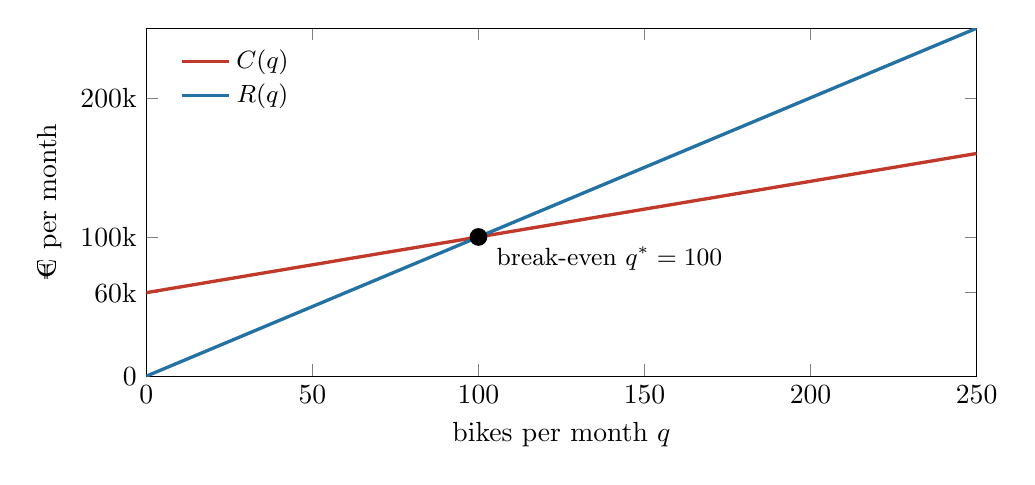
\begin{tikzpicture}
    \begin{axis}[width=\textwidth,height=6cm,xlabel={bikes per month $q$},ylabel={\texteuro\ per month},
      xmin=0,xmax=250,ymin=0,ymax=250000,ytick={0,60000,100000,200000},
      yticklabels={0,60k,100k,200k},xtick={0,50,100,150,200,250},legend pos=north west,legend style={draw=none,font=\small},grid=none]
      \addplot[brick,very thick,domain=0:250] {60000+400*x}; \addlegendentry{$C(q)$}
      \addplot[navy,very thick,domain=0:250] {1000*x}; \addlegendentry{$R(q)$}
      \addplot[only marks,mark=*,mark size=3pt,black] coordinates {(100,100000)};
      \node[anchor=north west,font=\small,xshift=3pt] at (axis cs:100,100000) {break-even $q^{*}=100$};
    \end{axis}
    \end{tikzpicture}
  \end{column}
  \begin{column}{0.45\textwidth}
    \[ 1{,}000\,q = 60{,}000 + 400\,q \]
    \[ 600\,q = 60{,}000 \]
    \[ q^{*} = \frac{60{,}000}{600} = 100 \]
    \vspace{0.3em}
    \textbf{Reading.} \texteuro 600 is the \emph{contribution} of each bike. Break-even is fixed cost $\div$ contribution.
  \end{column}
  \end{columns}
\end{frame}

\labframe{\S A}{Move the price. Then raise the rent.}{%
  \begin{enumerate}
    \item Bet: what price makes break-even 50 bikes? Then slide.
    \item The landlord raises fixed cost to \texteuro 72{,}000. Before running: what happens to the cost line, and to the crossing?
  \end{enumerate}
  \vspace{0.6em}
  Watch the \emph{slope} and the \emph{intercept} separately. Only one of them moved.}

\begin{frame}{A cost shock is a parallel shift --- remember this for the midterm}
  \begin{columns}
  \begin{column}{0.55\textwidth}
    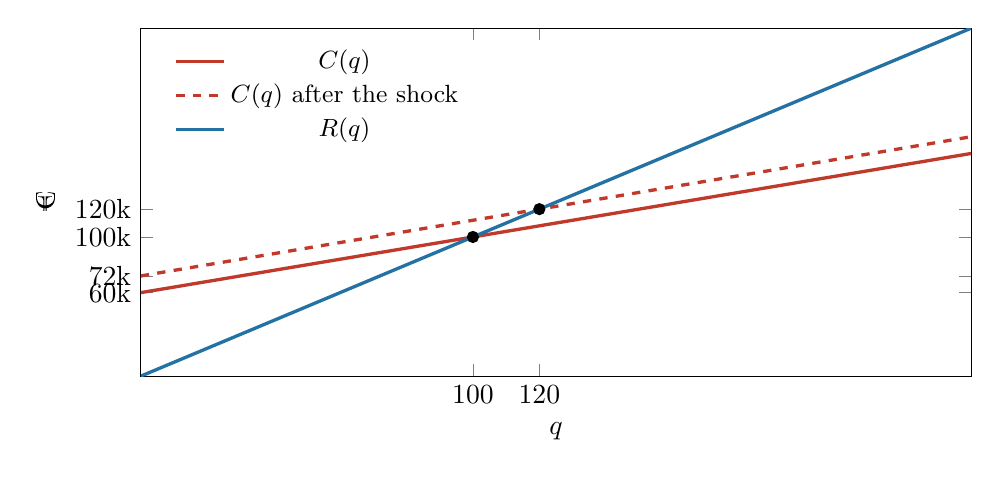
\begin{tikzpicture}
    \begin{axis}[width=\textwidth,height=6cm,xlabel={$q$},ylabel={\texteuro},xmin=0,xmax=250,ymin=0,ymax=250000,
      ytick={60000,72000,100000,120000},yticklabels={60k,72k,100k,120k},xtick={100,120},legend pos=north west,legend style={draw=none,font=\small}]
      \addplot[brick,very thick,domain=0:250] {60000+400*x}; \addlegendentry{$C(q)$}
      \addplot[brick,very thick,dashed,domain=0:250] {72000+400*x}; \addlegendentry{$C(q)$ after the shock}
      \addplot[navy,very thick,domain=0:250] {1000*x}; \addlegendentry{$R(q)$}
      \addplot[only marks,mark=*,black] coordinates {(100,100000) (120,120000)};
    \end{axis}
    \end{tikzpicture}
  \end{column}
  \begin{column}{0.45\textwidth}
    Same slope (\texteuro 400 per bike), higher intercept.\\[0.4em]
    New break-even: $1{,}000q = 72{,}000 + 400q \Rightarrow q^{*} = 120$.\\[0.8em]
    \alert{The midterm asks how a tariff on an input changes the cost and profit \emph{schedules}. That is this picture with different names: a per-unit tariff changes the slope, a lump-sum cost changes the intercept.}
  \end{column}
  \end{columns}
\end{frame}

\begin{frame}{The whole market: two facts, two unknowns}
  Buyers in Tuscany: $Q_d = 1200 - 2p$. \quad Sellers: $Q_s = -300 + 3p$.
  \bet{What price clears the market?}
  \begin{columns}[T]
  \begin{column}{0.33\textwidth}
    \textbf{Substitution}\\
    $1200 - 2p = -300 + 3p$\\
    $1500 = 5p$\\
    $p^{*} = 300$, $Q^{*} = 600$
  \end{column}
  \begin{column}{0.33\textwidth}
    \textbf{Elimination}\\
    $Q + 2p = 1200$\\
    $Q - 3p = -300$\\
    subtract: $5p = 1500$
  \end{column}
  \begin{column}{0.33\textwidth}
    \textbf{Picture}\\
    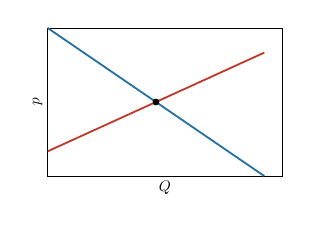
\begin{tikzpicture}[scale=0.55]
    \begin{axis}[width=7cm,height=5cm,xlabel={$Q$},ylabel={$p$},xmin=0,xmax=1300,ymin=0,ymax=600,ticks=none]
      \addplot[navy,very thick,domain=0:600] ({1200-2*x},{x});
      \addplot[brick,very thick,domain=100:500] ({-300+3*x},{x});
      \addplot[only marks,mark=*,black] coordinates {(600,300)};
    \end{axis}
    \end{tikzpicture}
  \end{column}
  \end{columns}
  \vspace{0.3em}
  \board{One equation is one fact about the business. Two unknowns need two facts. Write the facts as equations before touching a number.}
\end{frame}

\paperframe{D1, D2 (core) --- D3 (stretch)}{10}

% ================================================================== B
\section{B. How many bikes? --- quadratics}

\begin{frame}{Price responds to volume}
  The founder learns: at \texteuro 1{,}000 she sells 150 bikes; every \texteuro 4 cut sells one more.
  \[ p(q) = 1600 - 4q \]
  Revenue is \textbf{price $\times$ quantity}: a rectangle whose sides pull in opposite directions.
  \bet{Does selling more \emph{always} bring more revenue? Yes / no, and roughly where it stops.}
\end{frame}

\clipframe{w01_parabola}{%
  \only<1>{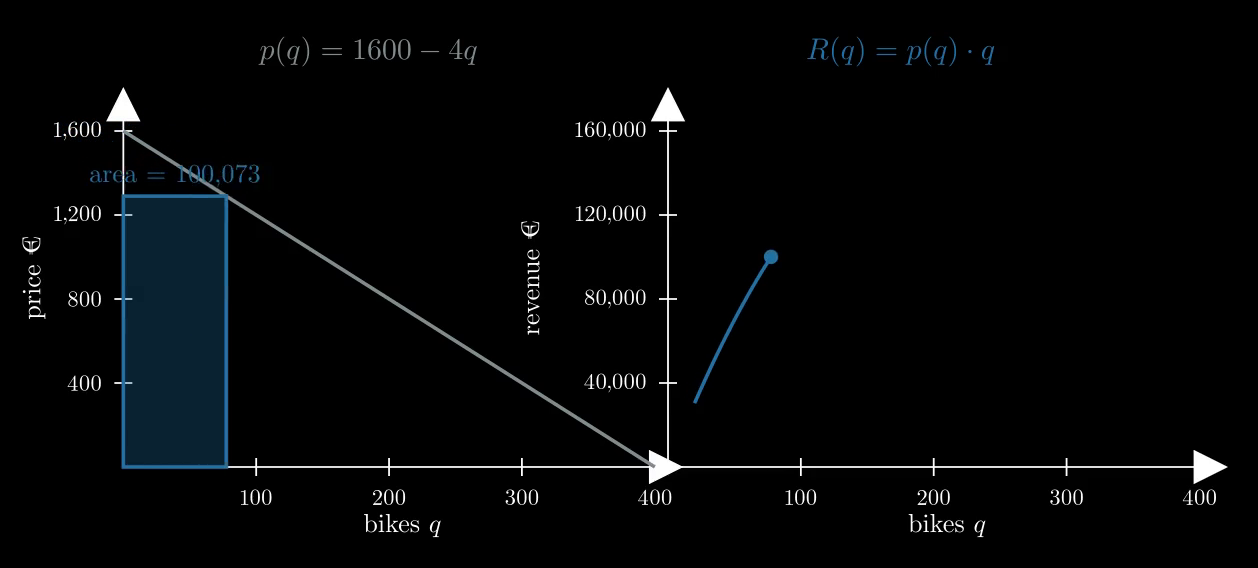
\includegraphics[width=\textwidth,height=0.82\textheight,keepaspectratio]{../../anim/frames/w01_parabola_1.png}}%
  \only<2>{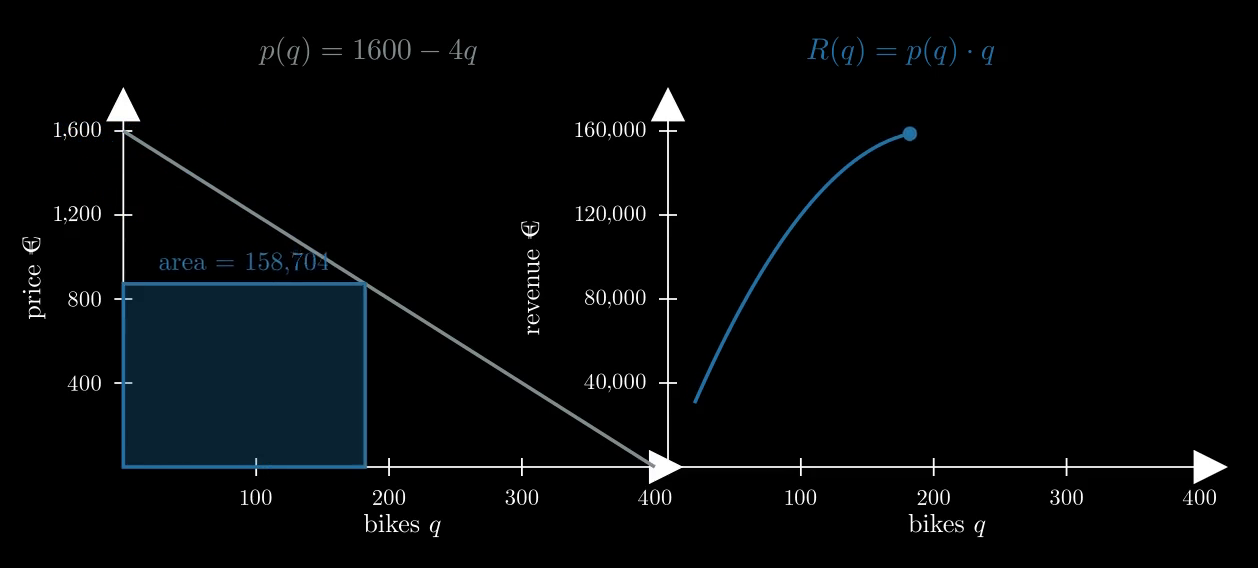
\includegraphics[width=\textwidth,height=0.82\textheight,keepaspectratio]{../../anim/frames/w01_parabola_2.png}}%
  \only<3>{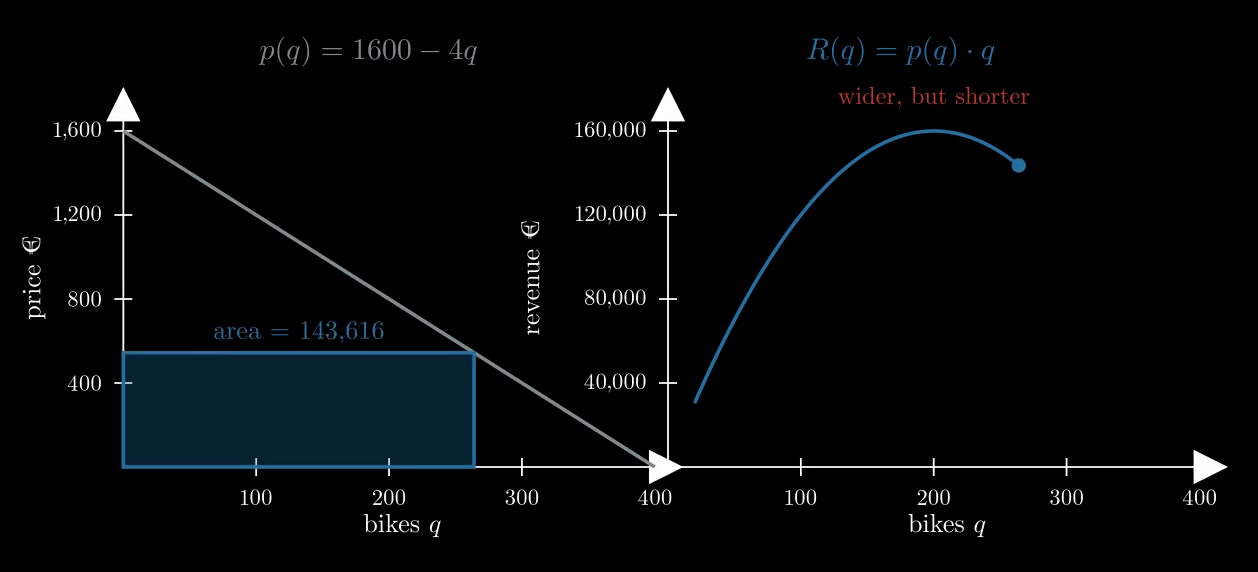
\includegraphics[width=\textwidth,height=0.82\textheight,keepaspectratio]{../../anim/frames/w01_parabola_3.png}}%
  \only<4>{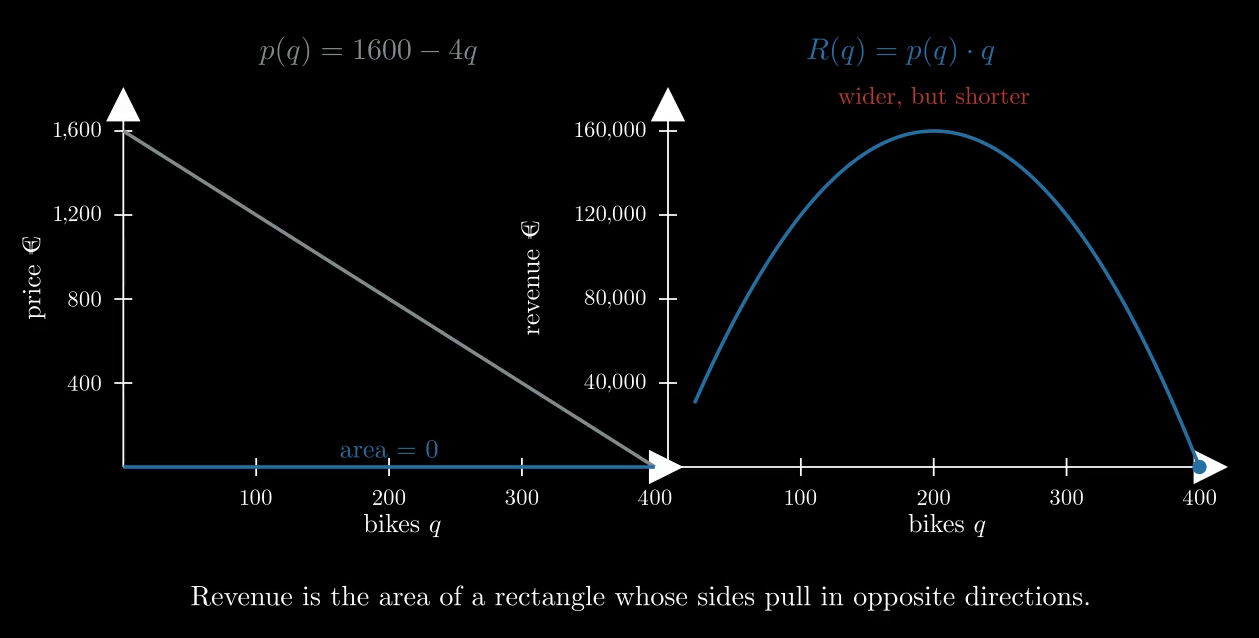
\includegraphics[width=\textwidth,height=0.82\textheight,keepaspectratio]{../../anim/frames/w01_parabola_4.png}}}{w01_parabola.mp4}

\begin{frame}{Revenue, cost, profit}
  \[ R(q) = (1600 - 4q)\,q = 1600q - 4q^{2} \]
  \[ \pi(q) = R(q) - C(q) = -4q^{2} + 1200q - 60{,}000 \]
  \pause
  \textbf{Where is profit zero?} First move, always: divide out the common factor.
  \[ q^{2} - 300q + 15{,}000 = 0 \]
  \[ q = \frac{300 \pm \sqrt{300^{2} - 4\cdot 15{,}000}}{2} = \frac{300 \pm \sqrt{30{,}000}}{2} \approx 63.4,\;\; 236.6 \]
\end{frame}

\begin{frame}{The discriminant decides before you compute}
  \begin{columns}[T]
  \begin{column}{0.5\textwidth}
    \begin{tabular}{@{}lll@{}}\toprule
    $b^{2} - 4ac$ & roots & in business \\ \midrule
    $> 0$ & two & a profitable window \\
    $= 0$ & one & a single break-even \\
    $< 0$ & none & no viable scale \\ \bottomrule
    \end{tabular}
    \vspace{1em}

    \textbf{Where is profit positive?} A downward parabola ($a<0$) is positive \emph{between} its roots:
    \[ 63.4 < q < 236.6 \]
  \end{column}
  \begin{column}{0.5\textwidth}
    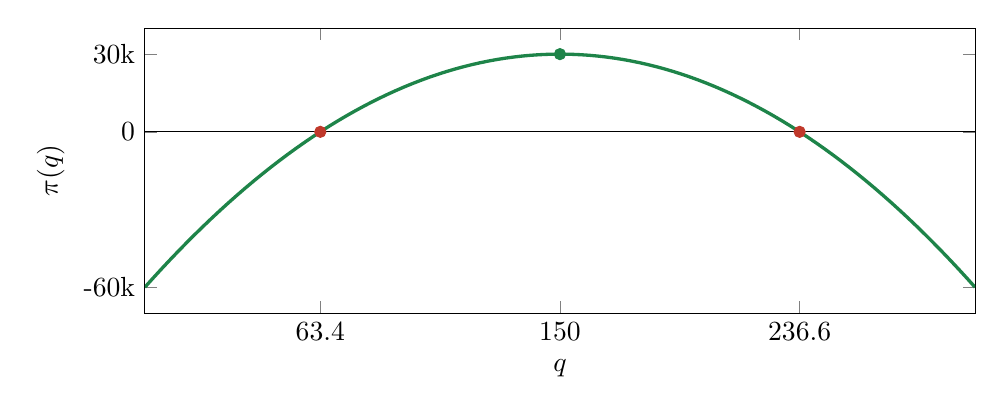
\begin{tikzpicture}
    \begin{axis}[width=\textwidth,height=5.2cm,xlabel={$q$},ylabel={$\pi(q)$},xmin=0,xmax=300,ymin=-70000,ymax=40000,
      ytick={-60000,0,30000},yticklabels={-60k,0,30k},xtick={63.4,150,236.6},xticklabels={63.4,150,236.6}]
      \addplot[leaf,very thick,domain=0:300,samples=100] {-4*x^2+1200*x-60000};
      \addplot[black,thin,domain=0:300] {0};
      \addplot[only marks,mark=*,brick] coordinates {(63.4,0) (236.6,0)};
      \addplot[only marks,mark=*,leaf] coordinates {(150,30000)};
    \end{axis}
    \end{tikzpicture}
    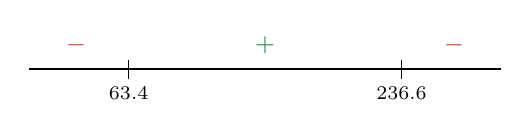
\begin{tikzpicture}[xscale=0.02]
      \draw[thick] (0,0) -- (300,0);
      \foreach \x in {63.4,236.6} \draw (\x,-0.12) -- (\x,0.12);
      \node[font=\small,brick] at (30,0.3) {$-$}; \node[font=\small,leaf] at (150,0.3) {$+$}; \node[font=\small,brick] at (270,0.3) {$-$};
      \node[font=\scriptsize,below] at (63.4,-0.1) {63.4}; \node[font=\scriptsize,below] at (236.6,-0.1) {236.6};
    \end{tikzpicture}\\
    {\small The sign line. In the midterm it is called ``the sign of the profit function''.}
  \end{column}
  \end{columns}
\end{frame}

\labframe{\S B}{Push the fixed cost up. Where do the two break-evens merge?}{%
  \begin{enumerate}
    \item Bet on the fixed cost at which the roots become one. (Hint: what is the profit at the vertex now?)
    \item Then push further. What does ``no roots'' look like, and what does it mean for the founder?
  \end{enumerate}}

\begin{frame}{The top of the hill, for now}
  Vertex of $\pi(q) = -4q^{2} + 1200q - 60{,}000$:
  \[ q_{v} = -\frac{b}{2a} = -\frac{1200}{-8} = 150 \qquad \pi(150) = 30{,}000 \]
  \vspace{0.3em}
  This formula works for parabolas only.\\[0.4em]
  \alert{Next week you get a tool that finds the top of the hill for \emph{any} curve --- a log revenue, a cubic cost, anything. It is called the derivative, and it is the reason this course exists.}
  \board{A quadratic has two roots, one, or none, and the discriminant tells you which before you compute. In business: a profitable window, a single break-even, no viable scale.}
\end{frame}

\paperframe{D4, D5 (core) --- D6 (stretch: factor and cancel)}{10}

% ================================================================== C
\section{C. How long to double? --- exponentials and logarithms}

\begin{frame}{Revenue \texteuro 1.2M, growing 12\% a year}
  \[ R(t) = 1.2 \cdot 1.12^{\,t} \]
  Linear growth adds the same \textbf{amount} each year. Exponential growth adds the same \textbf{percentage}.
  \bet{How many years to double? Write a number.}
\end{frame}

\clipframe{w01_growth}{%
  \only<1>{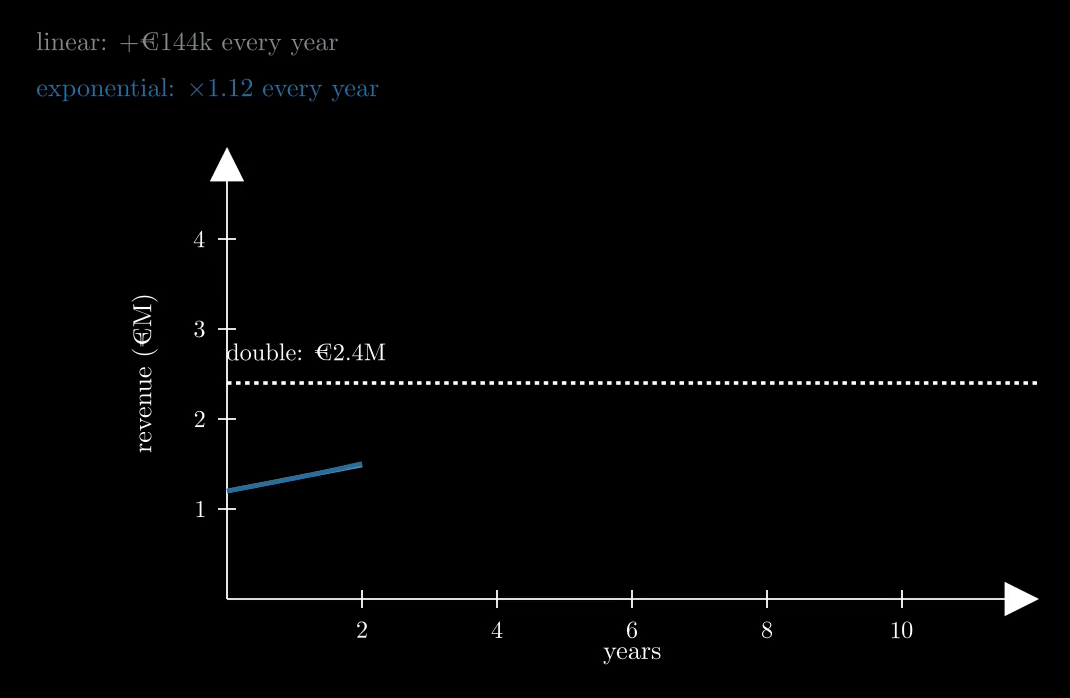
\includegraphics[width=\textwidth,height=0.82\textheight,keepaspectratio]{../../anim/frames/w01_growth_1.png}}%
  \only<2>{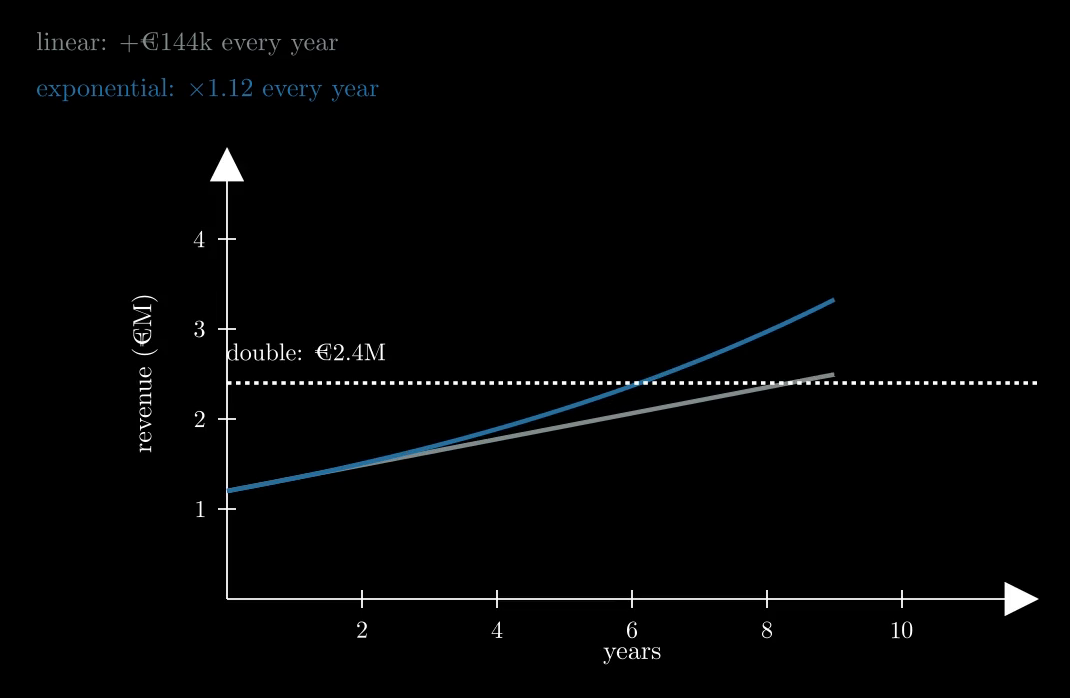
\includegraphics[width=\textwidth,height=0.82\textheight,keepaspectratio]{../../anim/frames/w01_growth_2.png}}%
  \only<3>{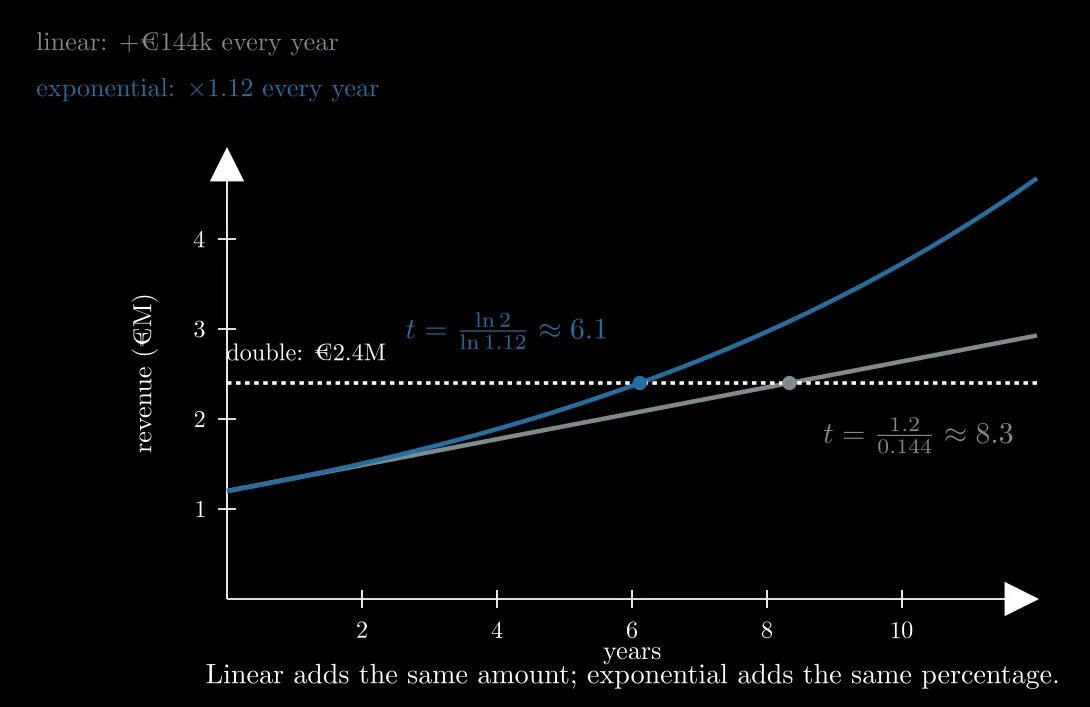
\includegraphics[width=\textwidth,height=0.82\textheight,keepaspectratio]{../../anim/frames/w01_growth_3.png}}}{w01_growth.mp4}

\begin{frame}{The unknown is in the exponent}
  \vspace{-0.6em}\[ 1.2 \cdot 1.12^{\,t} = 2.4 \quad\Longrightarrow\quad 1.12^{\,t} = 2 \]
  No algebra so far reaches $t$. \textbf{That is what a logarithm is for:} it answers ``to what power?''
  \pause
  \[ \ln\!\left(1.12^{\,t}\right) = \ln 2 \quad\Longrightarrow\quad t\,\ln 1.12 = \ln 2 \quad\Longrightarrow\quad t = \frac{0.6931}{0.1133} \approx 6.1 \text{ years} \]
  \pause
  \begin{center}\small
  \begin{tabular}{@{}ll@{}}\toprule
    rule & reading \\ \midrule
    $\ln(ab) = \ln a + \ln b$ & growth factors multiply, their logs add \\
    $\ln(a/b) = \ln a - \ln b$ & a ratio of revenues becomes a difference \\
    $\ln a^{k} = k \ln a$ & $k$ years of the same growth: the exponent comes down \\
    $\log_{b} x = \ln x / \ln b$ & any base through the calculator's $\ln$ \\ \bottomrule
  \end{tabular}
  \end{center}
\end{frame}

\begin{frame}{The sanity check you will use in the exam}
  \[ t_{\text{double}} \approx \frac{70}{g_{\%}} \qquad\qquad \frac{70}{12} \approx 5.8 \]
  Why it works: $\ln 2 \approx 0.69$ and $\ln(1+g) \approx g$ when $g$ is small, so $t = \ln 2 / \ln(1+g) \approx 0.69/g$.\\[0.8em]
  The number $e \approx 2.718$ appears today only as ``the base your calculator's $\ln$ uses''. In week 4 it becomes continuous compounding and earns its place.
  \board{Whenever the unknown is in the exponent, take logs of both sides. Whenever you see a log, remember it is a question: to what power?}
\end{frame}

\paperframe{D7, D8 (core) --- D9 (stretch: $5e^{0.03t} = 8$)}{12}

% ================================================================== D
\section{D. Within tolerance --- absolute value}

\begin{frame}{Is this cell within spec?}
  Battery cells must be $500\,\text{Wh} \pm 15$. A supplier ships one at 483 Wh.
  \bet{In or out? Then write the rule as one inequality.}
  \pause
  \[ |c - 500| \le 15 \;\Longleftrightarrow\; 485 \le c \le 515 \;\Longleftrightarrow\; c \in [485,\,515] \]
  \begin{center}
  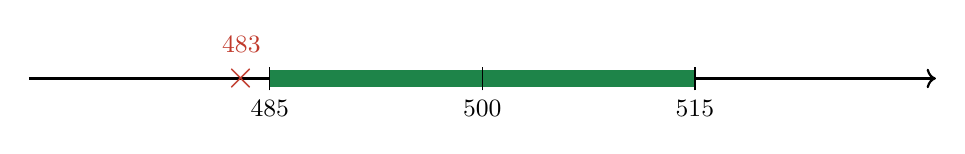
\begin{tikzpicture}[xscale=0.18]
    \draw[thick,->] (468,0) -- (532,0);
    \draw[leaf,line width=6pt] (485,0) -- (515,0);
    \foreach \x/\l in {485/485,500/500,515/515} {\draw (\x,-0.15)--(\x,0.15); \node[below,font=\small] at (\x,-0.15) {\l};}
    \node[brick,font=\Large] at (483,0) {$\times$}; \node[above,brick,font=\small] at (483,0.2) {483};
  \end{tikzpicture}
  \end{center}
  \vspace{-0.4em}{\small $|x-a|$ is the \textbf{distance} from $a$. ``$\le b$'' is the closed interval $[a-b,\,a+b]$; ``$> b$'' is the two tails $x<a-b$ or $x>a+b$.\\[0.4em]
  Square bracket: endpoint included. Round bracket: excluded, or $\pm\infty$. The exam asks for domains written exactly like this.}
\end{frame}

\paperframe{D10, D11 (core) --- interval notation}{8}

% ================================================================== close
\section{Board pitch and close}

\begin{frame}{Sixty seconds to the Board}
  One of you stands up. The other is the Board.\\[0.6em]
  Tell them, with numbers and no formulas:
  \begin{itemize}
    \item where Arno Bikes breaks even at today's price;
    \item between which volumes it makes money once price responds to volume, and how fragile that window is;
    \item how long until revenue doubles at 12\%.
  \end{itemize}
  \vspace{0.4em}
  The Board asks one question. \hfill {\small This is a rehearsal of the midterm's oral.}
\end{frame}

\begin{frame}{Take home}
  \begin{enumerate}
    \item Write the facts as equations before touching numbers.
    \item Discriminant first, then roots, then the sign line.
    \item Unknown in the exponent $\rightarrow$ take logs of both sides.
  \end{enumerate}
  \vspace{0.8em}
  \textbf{Homework 1} (\texttt{homework.md}), due Wednesday 30 Sep 23:59 on Moodle: eight drills on paper + a 150--250-word memo to the Board on the profitable window.\\[0.6em]
  Write your own three take-home lines now, before you leave.
\end{frame}

\end{document}
